\chapter{Experiment Description}

\section{The Large Hadron Collider (LHC)}

\section{The Compact Muon Solenoid (CMS)}

\subsection{Superconducting Magnet}

\subsection{Tracker}

\subsection{Electromagnetic Calorimeter (ECAL)}

\subsection{Hadronic Calorimeter (HCAL)}

\subsection{Muon Detectors}

\begin{figure}
  \centering
   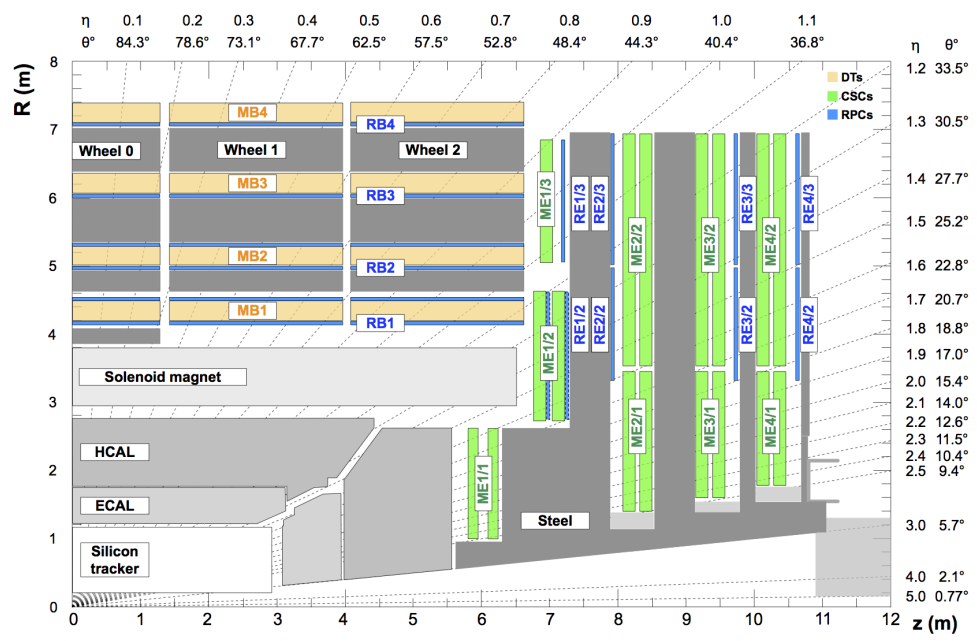
\includegraphics[width=0.9\textwidth]{fig/experiment/detector/muon_sys_r-z.png}
	\caption{Diagram of CMS detector in the r-z plane showing the components of the muon system.}
\end{figure}

\section{Trigger System}

\section{Object Reconstruction}
The global event reconstruction (also called particle-flow (PF) event reconstruction~\cite{CMS:2017yfk}) aims to reconstruct and identify each individual particle in an event, with an optimized combination of all subdetector information. In this process, the identification of the particle type (photon, electron, muon, charged hadron, neutral hadron) plays an important role in the determination of the particle direction and energy.

\begin{figure}
  \centering
   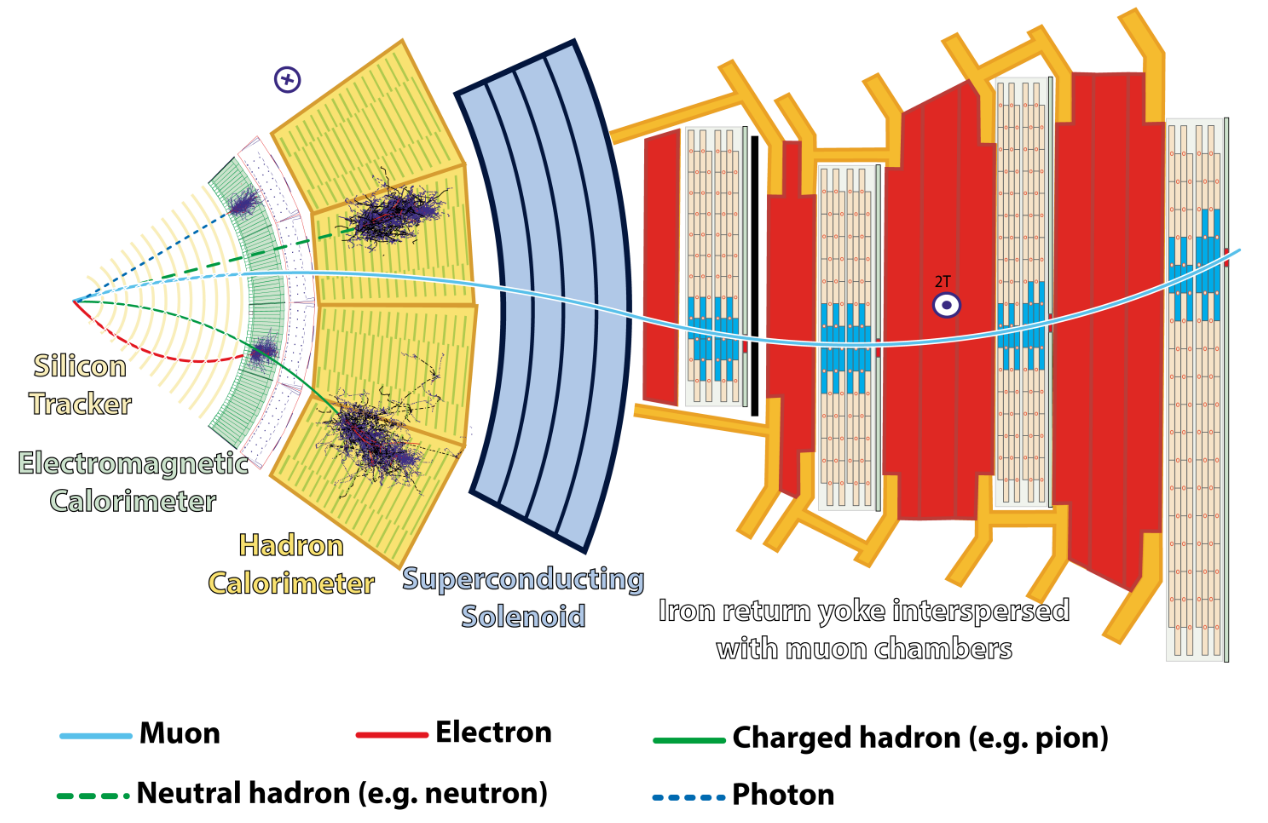
\includegraphics[width=0.9\textwidth]{fig/experiment/reconstruction/cms_detector.png}
	\caption{Schematic of different particles interacting with the CMS detector.}
\end{figure}

\subsection{Photon and Electron Reconstruction}
Photons and electrons interact with the material in the ECAL, depositing the majority of their energy before reaching the HCAL. As they interact, photons convert into 
electron-positron pairs and electrons radiate bremsstrahlung photons. This leads to the formation of an electromagnetic shower. Because of this, the original particle energy 
is split into multiple energy deposits, which must be combined to reconstruct the original energy. Deposits in individual ECAL crystals are combined into clusters, 
and these clusters are in turn combined into superclusters. Two algorithms are used to generate superclusters: the so-called "mustache" algorithm, and the so-called "refined" algorithm.
The mustache algorithm defines a seed cluster with energy above a certain threshold, and then combines it with other clusters within a region of the eta-phi plane centered at the 
seed location. The refined algorithm uses the mustache superclusters as well as tracking information to extrapolate bremsstrahlung and conversion tracks to decide whether a cluster should belong 
to the supercluster. 

The distinction between photons and electrons is made using tracking information, where photons are associated with no tracks and electrons with tracks. The Gaussian Sum Filter (GSF) [REF] track 
fitting algorithm is used to identify and characterize tracks that might be associated with an electron. It first begins with a hit pattern in the tracker, which is used as a seed. This seed 
can either be tracker-driven, coming from the collection of generic tracks tested for mutual compatibility, or it can be ECAL-driven, where a mustache supercluster is compared in location with 
a collection of tracker hit patterns to determine if the supercluster is consistent with the trajectory indicated by the track. Electron seeds are then converted into reconstructed electron tracks. 
In the absence of any GSF electron tracks, a photon candidate is obtained. Additional separation between photons and electrons is obtained through further selection requirements. 
The measured energy resolution for electrons produced in $\PZ$ boson decays in  $\Pp\Pp$ collision data ranges from $2$--$5$\%, depending on electron pseudorapidity and energy loss through bremsstrahlung in the detector material~\cite{CMS:2020uim}.

\subsection{Muon Reconstruction}
Muon reconstruction utilizes information from the muon detectors and the tracker. First, detector hits in the CSCs, DTs, and RPCs are used to build standalone tracks using a Kalman-filter technique.
Subsequently, these standalone muon tracks are combined with tracker information via two algorithms. So-called "tracker muons" are reconstructed using an "inside-out" algorithm, which starts from 
tracker tracks and matches them to DT or CSC segments. So-called "global muons" are reconstructed with an "outside-in" approach which starts from standalone muon tracks and matches them 
to tracker tracks using a Kalman-filter technique. In the case where both algorithms reconstruct a muon sharing the same tracker tack, the two outputs are merged into a single muon candidate.
In general, the tracker muon algorithm is more efficient in the region of low muon \pT, while the global algorithm is efficient at high \pT. 

The energy of muons is obtained from the corresponding track momentum. Matching muons to tracks measured in the silicon tracker results in a \pt resolution, for muons with \pt up to $100$\GeV, of $1$\% in the barrel and $3$\% in the endcaps. The \pt resolution in the barrel is better than $7$\% for muons with \pt up to $1$\TeV~\cite{CMS:2018rym}.


\subsection{Hadrons}

\subsection{Jets}

\begin{figure}
  \centering
   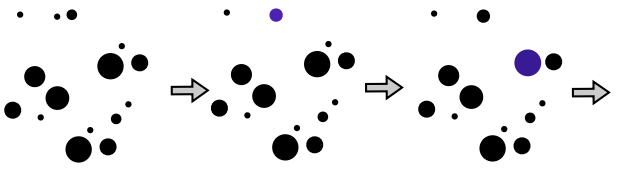
\includegraphics[width=0.9\textwidth]{fig/experiment/reconstruction/jet_clustering.png}
	\caption{Diagram representing the jet clustering algorithm.}
\end{figure}

\subsection{Primary Vertex}
